
\chapter{Diagramas do hardware}

\section{Diagrama de blocos}

Na figura \ref{fig:diagrama_blocos_hardware} mostra-se o diagrama de blocos do sistema embarcado e suas conexões com o restante do robô. A seguir está também uma descrição para cada um dos blocos da placa de circuito impresso do sistema embarcado.

\begin{figure}[htpb!]
  \centering
  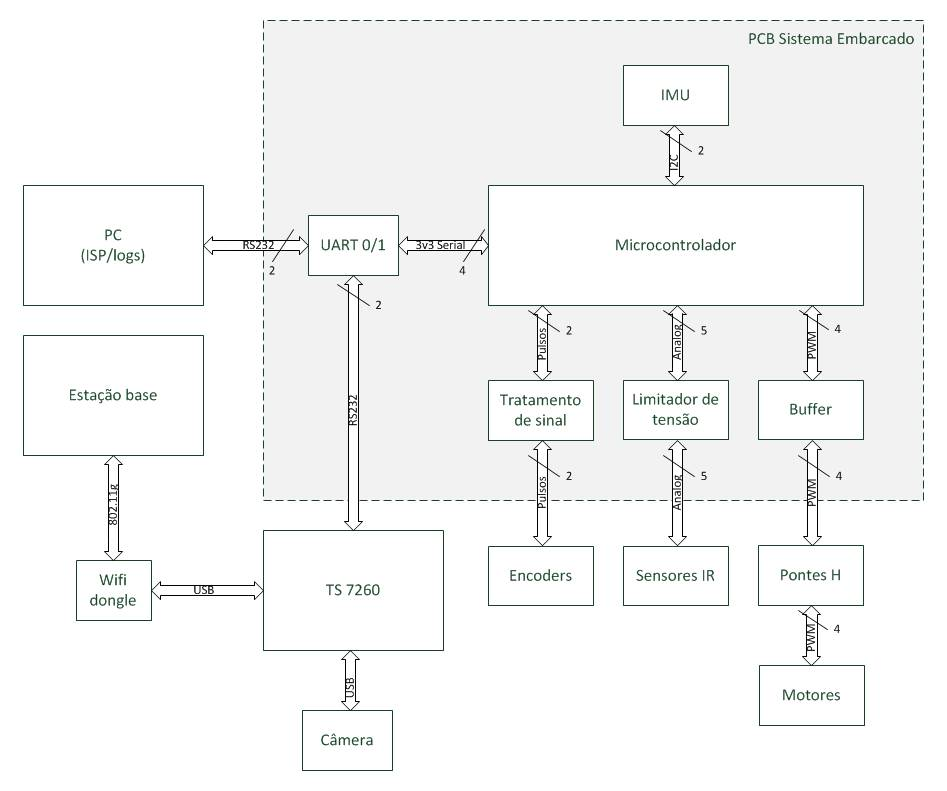
\includegraphics[width=\textwidth]{./figuras/diagrama_blocos_hardware.jpg}
  \caption{Diagrama de blocos do hardware}
  \label{fig:diagrama_blocos_hardware}
\end{figure}


\begin{enumerate}[topsep=0pt, partopsep=0pt, itemsep=0pt]
    \item Microcontrolador: Este bloco fará a leitura dos sensores: encoders, infra-vermelhos, acelerômetro e giroscópios. Além disso possui a implementação do protocolo de comunicação para interação com o linux embarcado da placa TS-7260.
    \item UART 0/1: Responsável por ajustar os níveis de tensão para comunicação serial no padrão RS-232 com a placa TS-7260.
    \item Buffer: Responsável por fornecer corrente e elevar os níveis de tensão de saída do microcontrolador de 3,3V para 5,0V. Esse buffer é conectado às pontes H já existentes no robô.
    \item IMU: possui o acelerômetro e o giroscópio e se comunicará com o microcontrolador por meio do protocolo I2C.
    \item Limitador de tensão: Necessário pois os sinais de saída dos sensores de infravermelho que já existem no robô não estão limitados em 5V, podendo a saída ultrapassar 5,0V e danificar o microcontrolador. 
    \item Tratamento de sinal: Composto por um filtro RC passa baixas e um schmitt trigger para remover qualquer falha que possa ocorrer na geração dos pulsos no encoder.
\end{enumerate}

\section{Diagrama elétrico/eletrônico}

Na figura \ref{fig:diagrama_eletrico_eletronico} mostra-se o diagrama de elétrico eletrônico do sistema embarcado. Cada bloco da figura \ref{fig:diagrama_blocos_hardware} corresponde a alguns componentes do diagrama elétrico eletrônico. A seguir detalha-se um pouco mais cada bloco.

\begin{figure}[htpb!]
  \centering
  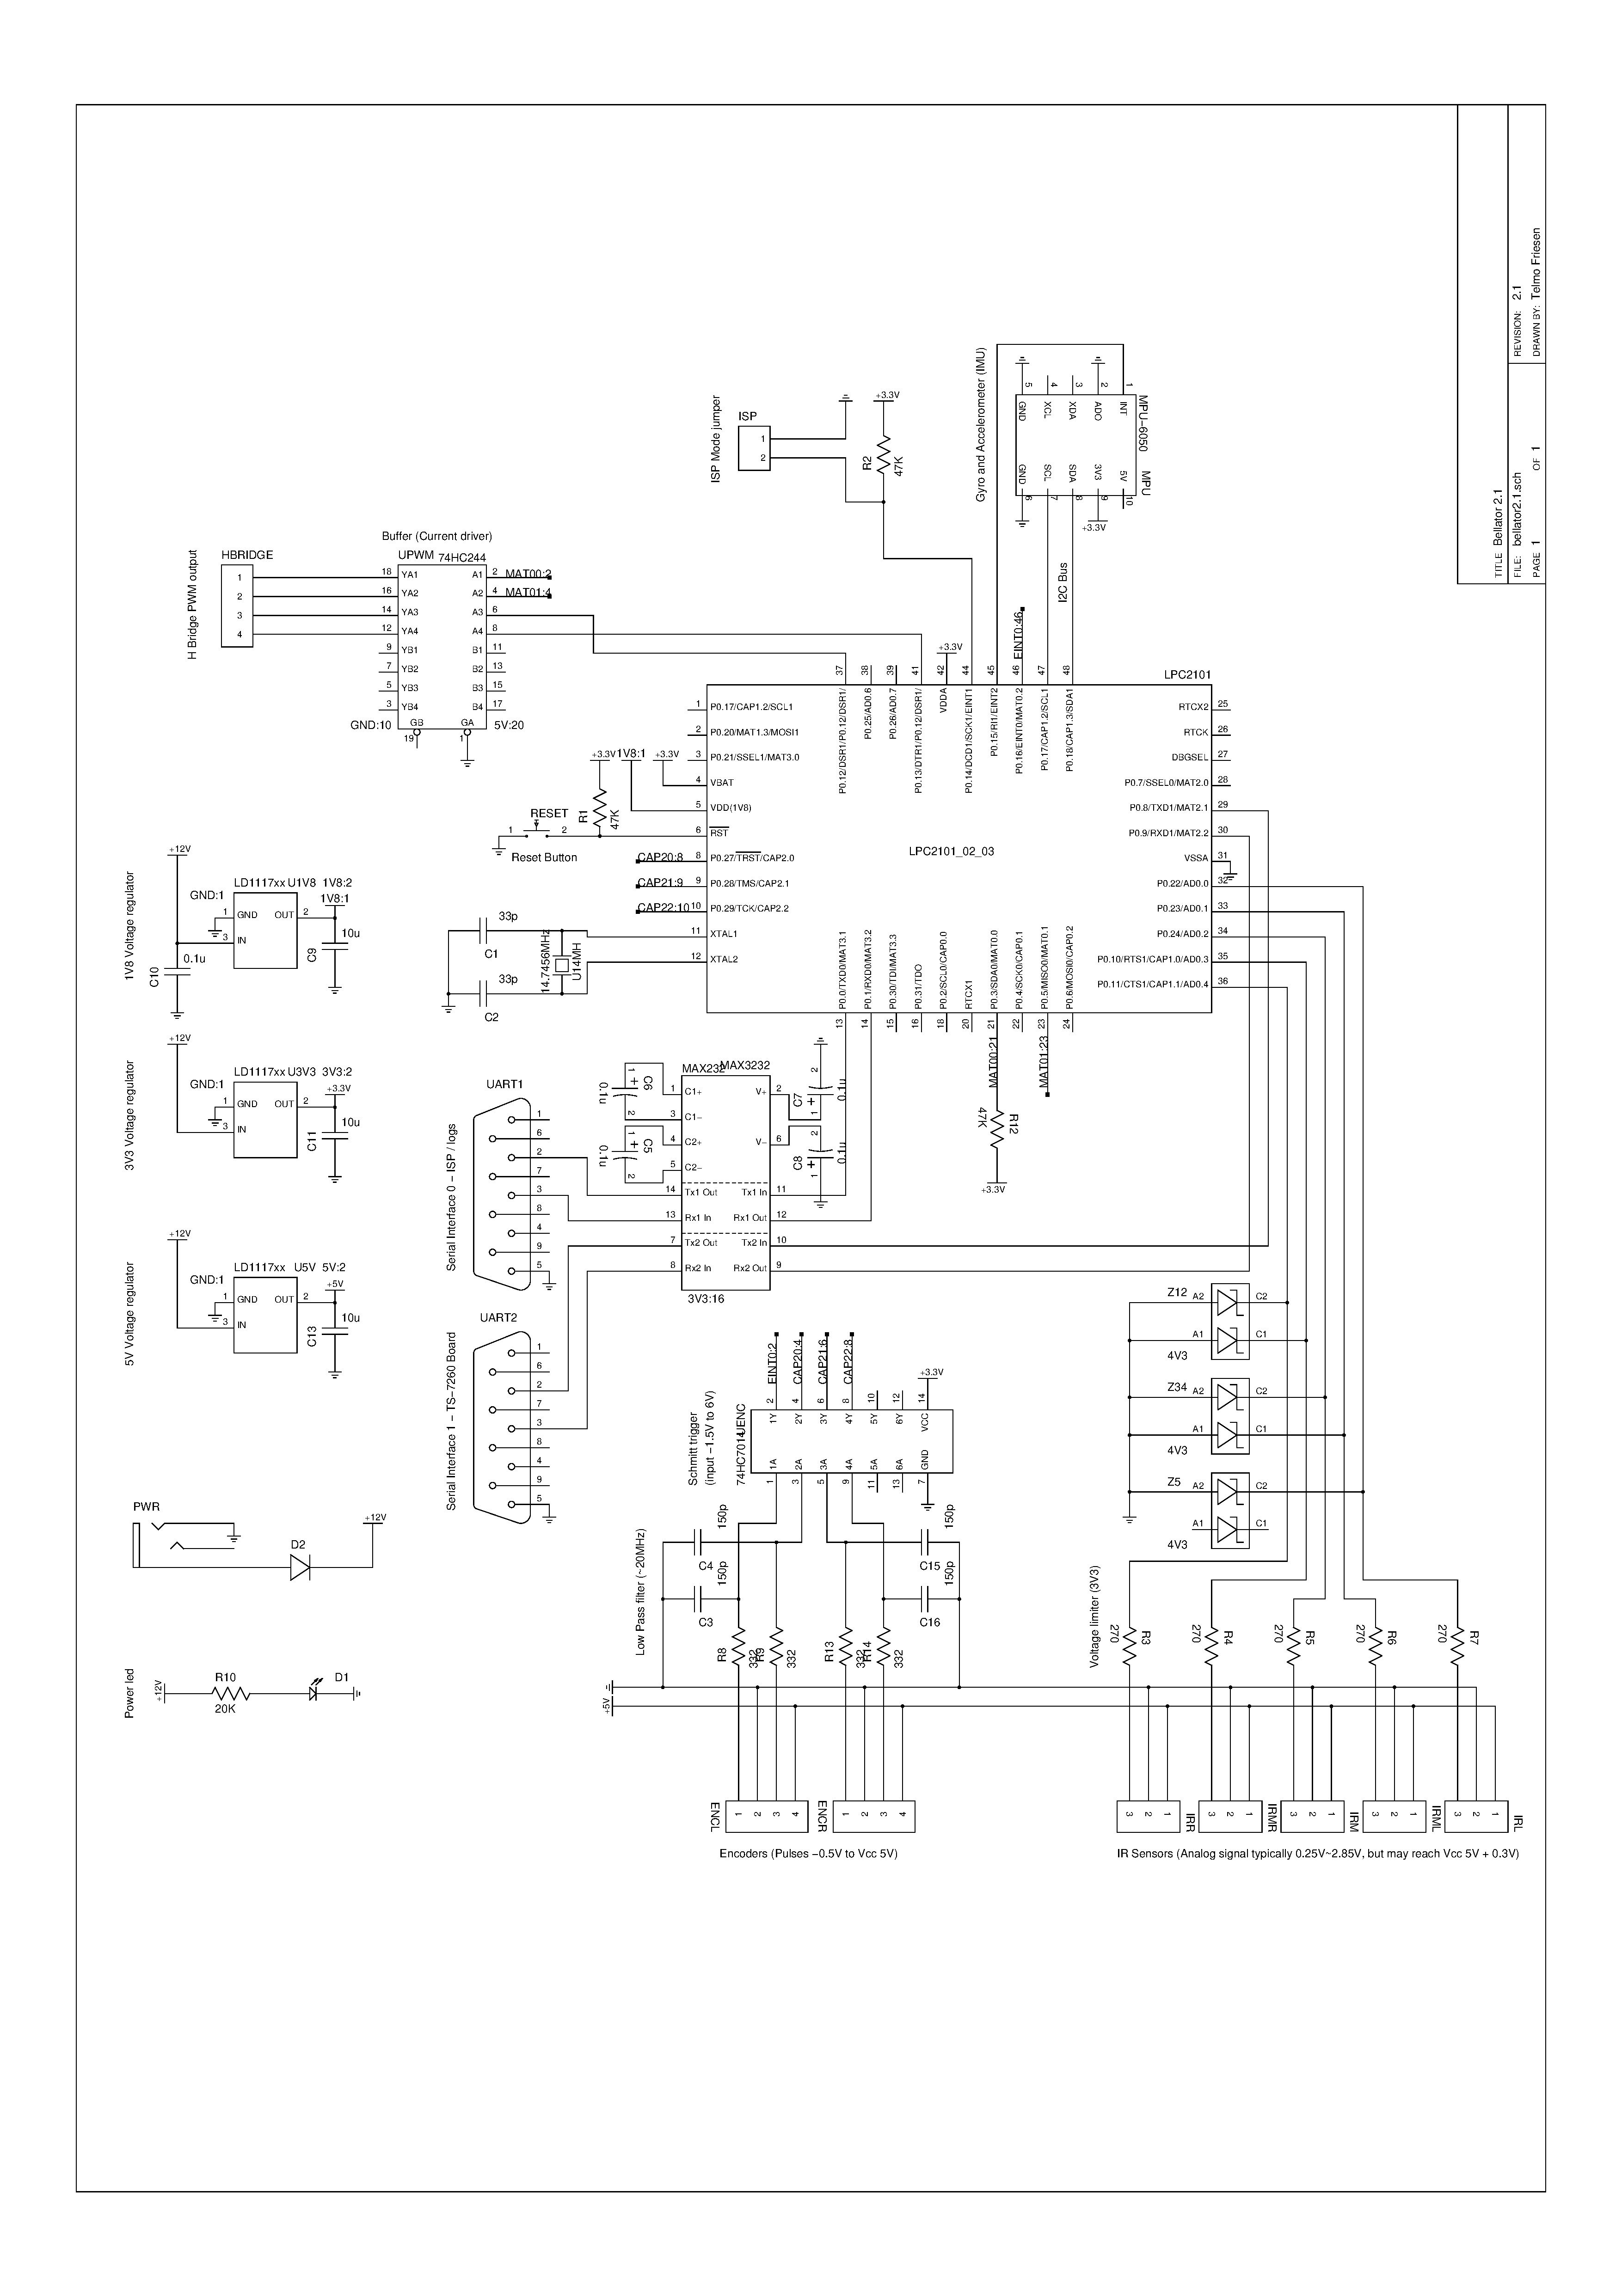
\includegraphics[width=0.9\textwidth, keepaspectratio]{./figuras/hardware2_2.pdf}
  \caption{Diagrama elétrico/eletrônico.}
  \label{fig:diagrama_eletrico_eletronico}
\end{figure}

\begin{enumerate}[topsep=0pt, partopsep=0pt, itemsep=0pt]
    \item Microcontrolador: Composto pelo microcontrolador LCP2103 da NXP que possui arquitetura ARM. Ele dispõe de duas interfaces seriais, conversor analógico digital com 8 canais, interface i2c, entradas de captura e interrupção, saídas de PWM entre outras funções que não serão utilizadas nesse projeto.
    \item UART 0/1: Constituído por um chip max3232 que opera em níveis de tensão CMOS e que gera os níveis adequados para o padrão RS-232 utilizando alguns capacitores.
    \item Buffer: Constituído por um chip 74HC244, é responsável por fornecer corrente e elevar os níveis de tensão de saída do microcontrolador de 3,3V para 5,0V.
    \item IMU: Composto pela placa de desenvolvimento MPU-6050, que possui um chip com o mesmo nome, MPU-6050, e circuitos RC auxiliares necessários para o funcionamento do MPU-6050.
    \item Limitador de tensão: Constituído de um resistor com baixo valor, 270 ohms, e um diodo Zener polarizado reversamente e com tensão de ruptura de 4.3V. Quando a tensão de entrada ultrapassar 4.3V o diodo passa a conduzir e mantém a tensão de 4.3V no resistor. O datasheet do microcontrolador sugere que se mantenha a impedância da carga menor que 40kohms, logo a adição de um resistor de 270 ohms pode ser desconsiderado com relação ao erro que possa causar na leitura do conversor. Um resistor de 270 ohms leva a uma corrente de 3.7mA quando a saída do sensor for 5.3V, que é o valor máximo previsto no datasheet.
    \item Tratamento de sinal: Composto por um filtro RC passa baixas e um chip 74HC7014. As frequências acima de 20MHz são atenuadas no sinal do encoder. Esse valor foi calculado com base na forma de onda da saída especificada no datasheet do encoder. Para tanto utilizam-se resistores de 332 ohms e capacitores de 150pF.
\end{enumerate}
